% Native editable composition from verified, unchanged IDE images.
\par
\begin{figure}[htbp]
  \centering
  \sbox0{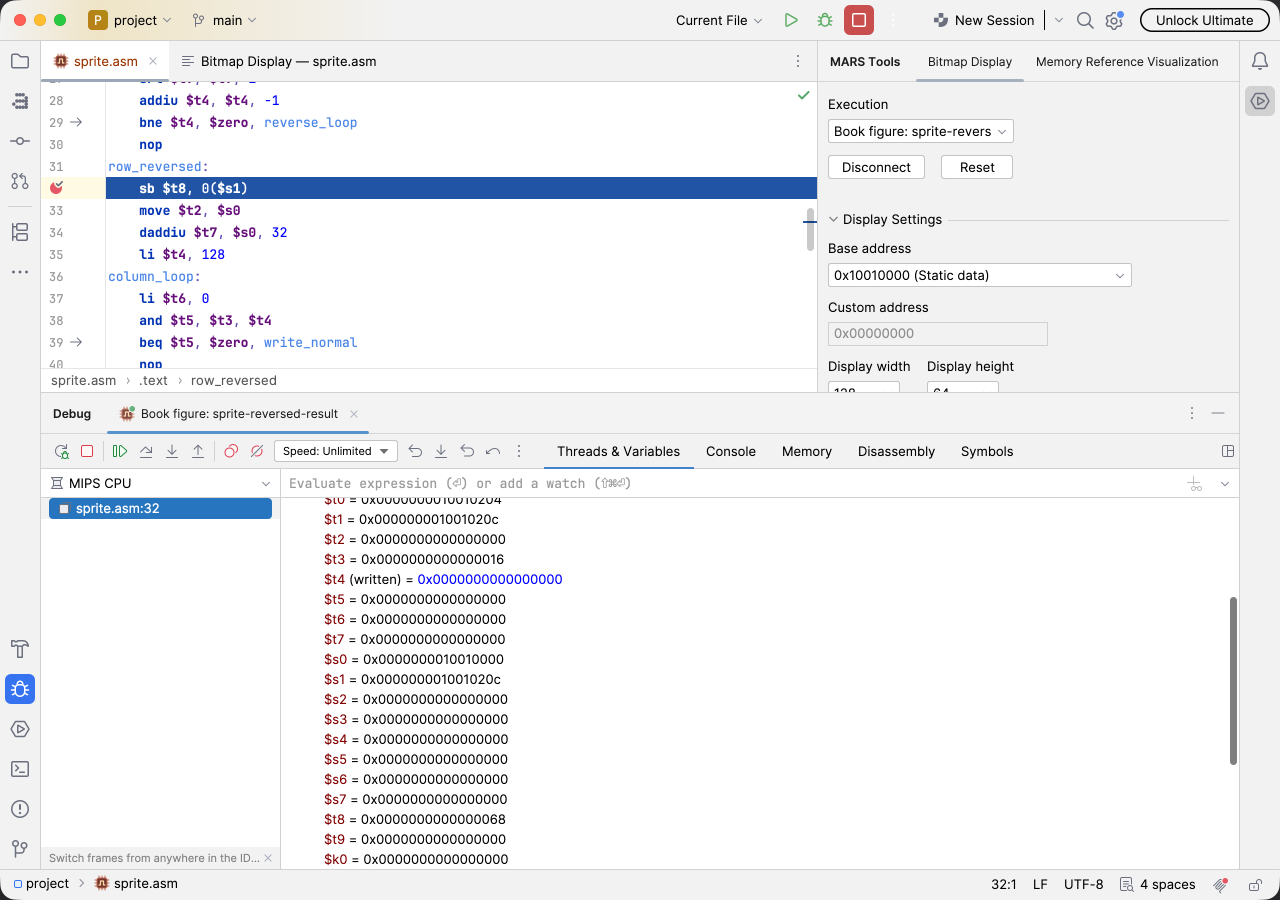
\includegraphics[artifact]{packages/003-eight-byte-sprite/captures/f02-reversal/result.png}}
  \sbox2{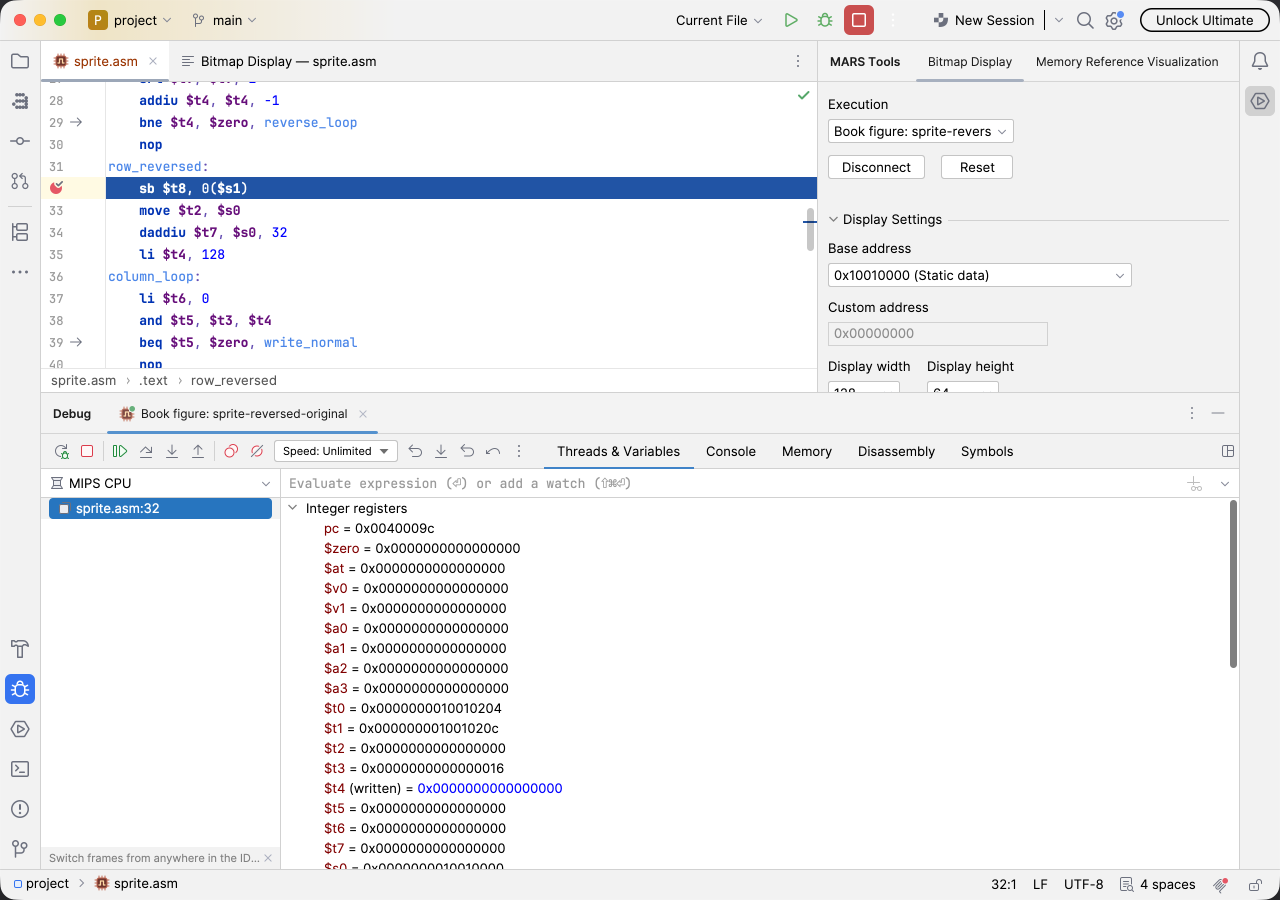
\includegraphics[artifact]{packages/003-eight-byte-sprite/captures/f02-reversal/original.png}}
  \sbox4{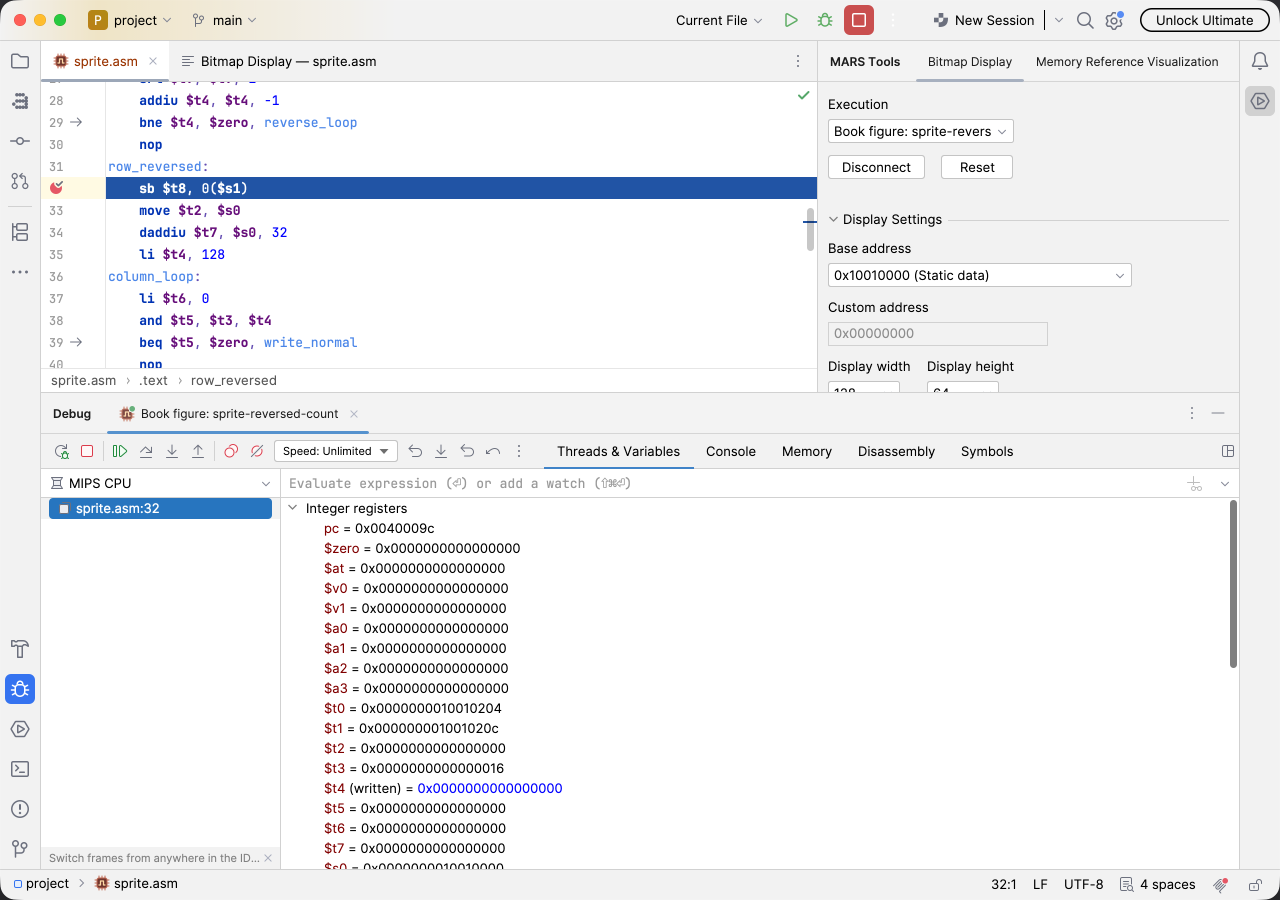
\includegraphics[artifact]{packages/003-eight-byte-sprite/captures/f02-reversal/count.png}}
  \edef\MARSreversedsourceLeft{\the\dimexpr0.036718750\wd0\relax}
  \edef\MARSreversedsourceBottom{\the\dimexpr0.774444444\ht0\relax}
  \edef\MARSreversedsourceRight{\the\dimexpr0.611718750\wd0\relax}
  \edef\MARSreversedsourceTop{\the\dimexpr0.172222222\ht0\relax}
  \edef\MARSreversedoriginalLeft{\the\dimexpr0.246093750\wd2\relax}
  \edef\MARSreversedoriginalBottom{\the\dimexpr0.132222222\ht2\relax}
  \edef\MARSreversedoriginalRight{\the\dimexpr0.600000000\wd2\relax}
  \edef\MARSreversedoriginalTop{\the\dimexpr0.838888889\ht2\relax}
  \edef\MARSreversedreversedLeft{\the\dimexpr0.246093750\wd0\relax}
  \edef\MARSreversedreversedBottom{\the\dimexpr0.075555556\ht0\relax}
  \edef\MARSreversedreversedRight{\the\dimexpr0.599218750\wd0\relax}
  \edef\MARSreversedreversedTop{\the\dimexpr0.895555556\ht0\relax}
  \edef\MARSreversedcountLeft{\the\dimexpr0.246093750\wd4\relax}
  \edef\MARSreversedcountBottom{\the\dimexpr0.110000000\ht4\relax}
  \edef\MARSreversedcountRight{\the\dimexpr0.554687500\wd4\relax}
  \edef\MARSreversedcountTop{\the\dimexpr0.861111111\ht4\relax}
  \begin{tikzpicture}[alt={Four annotated IDE details at row_reversed. The next instruction is sb t8 zero s1. Original register t3 is hexadecimal 16, reversed accumulator t8 is 68, and remaining iteration count t4 is zero. The original binary row 00010110 reverses to 01101000.}]
    \node[anchor=north west,inner sep=0,font=\small\bfseries] (source-title) at (6mm,0) {The reversed-byte store is next};
    \node[anchor=north west,inner sep=0] (source) at ([yshift=-1mm]source-title.south west) {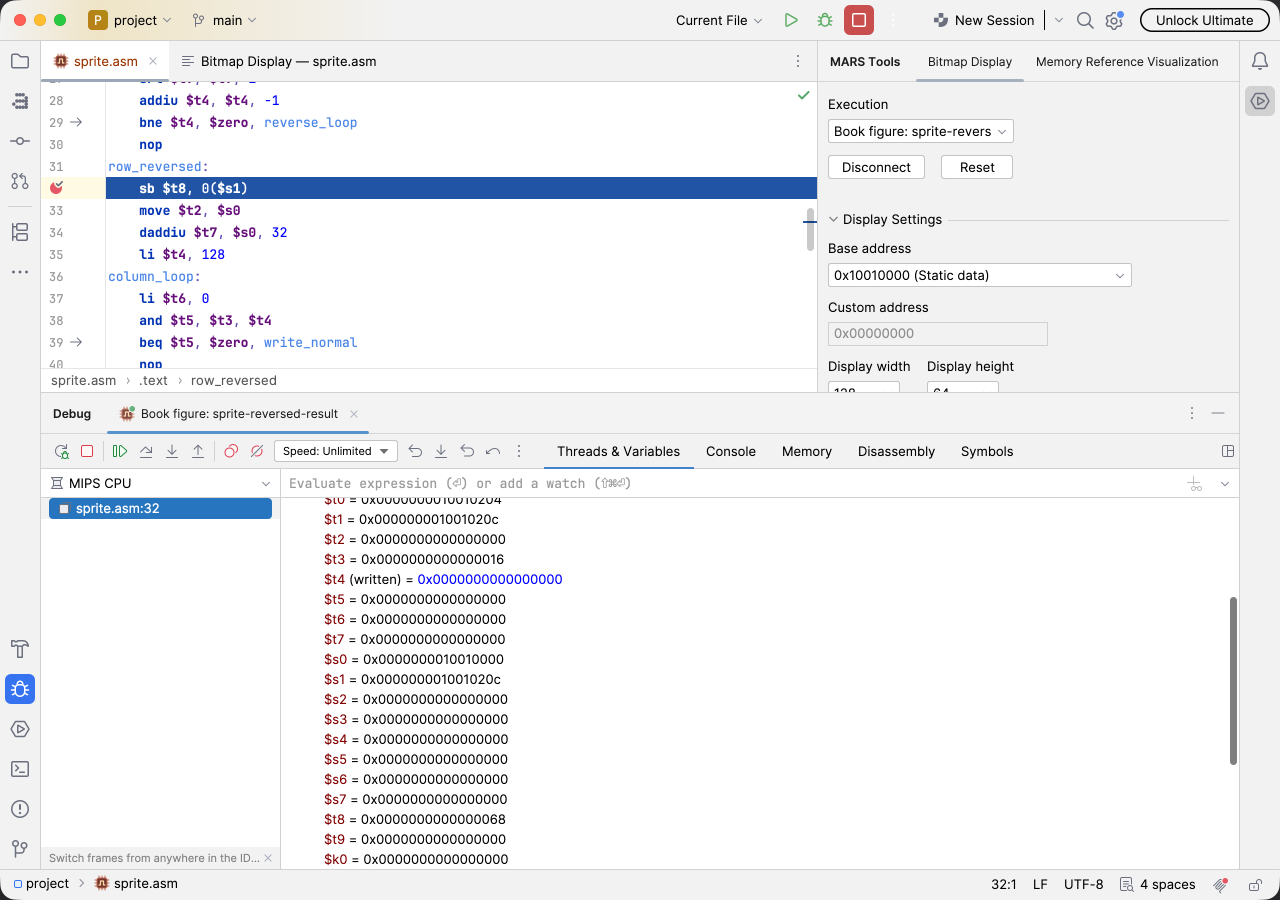
\includegraphics[width=0.7\linewidth,artifact,trim={\MARSreversedsourceLeft{} \MARSreversedsourceBottom{} \MARSreversedsourceRight{} \MARSreversedsourceTop{}},clip]{packages/003-eight-byte-sprite/captures/f02-reversal/result.png}};
    \begin{scope}[shift={(source.south west)},x={($(source.south east)-(source.south west)$)},y={($(source.north west)-(source.south west)$)}]
      \draw[black,line width=0.7pt] (0.135555556,0.083333333) rectangle (0.446666667,0.541666667);
      \node[draw=black,fill=white,circle,inner sep=1.5pt,font=\footnotesize] at ($(0.135555556,0.541666667)+(-3mm,0)$) {1};
    \end{scope}
    \node[anchor=north west,inner sep=0,font=\small\bfseries] (original-title) at ([yshift=-2mm]source.south west) {The preserved original row};
    \node[anchor=north west,inner sep=0] (original) at ([yshift=-1mm]original-title.south west) {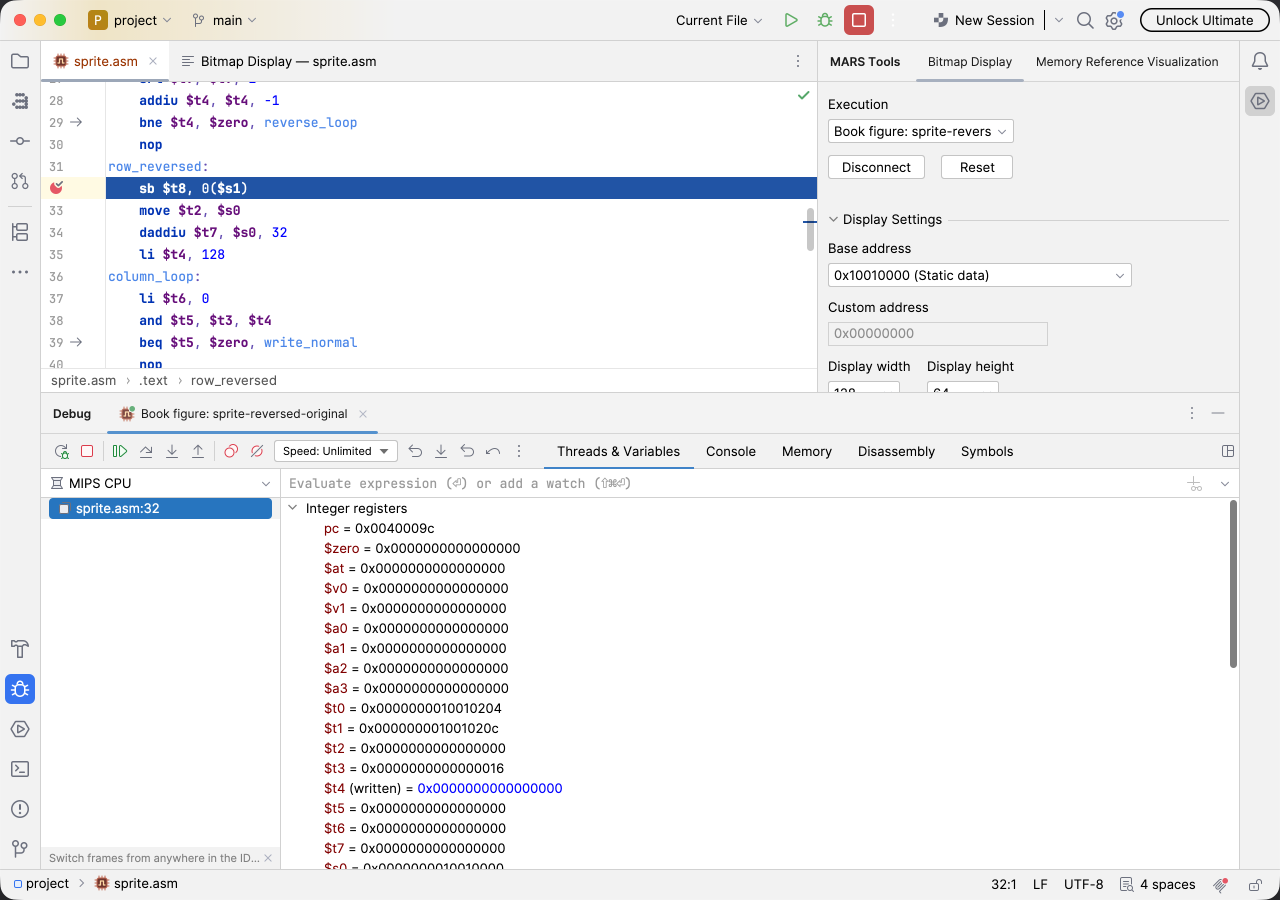
\includegraphics[width=0.53\linewidth,artifact,trim={\MARSreversedoriginalLeft{} \MARSreversedoriginalBottom{} \MARSreversedoriginalRight{} \MARSreversedoriginalTop{}},clip]{packages/003-eight-byte-sprite/captures/f02-reversal/original.png}};
    \begin{scope}[shift={(original.south west)},x={($(original.south east)-(original.south west)$)},y={($(original.north west)-(original.south west)$)}]
      \draw[black,line width=0.7pt] (0.030456853,0.115384615) rectangle (0.969543147,0.884615385);
      \node[draw=black,fill=white,circle,inner sep=1.5pt,font=\footnotesize] at ($(0.030456853,0.884615385)+(-3mm,0)$) {2};
    \end{scope}
    \node[anchor=north west,inner sep=0,font=\small\bfseries] (reversed-title) at ([yshift=-2mm]original.south west) {The completed reversed accumulator};
    \node[anchor=north west,inner sep=0] (reversed) at ([yshift=-1mm]reversed-title.south west) {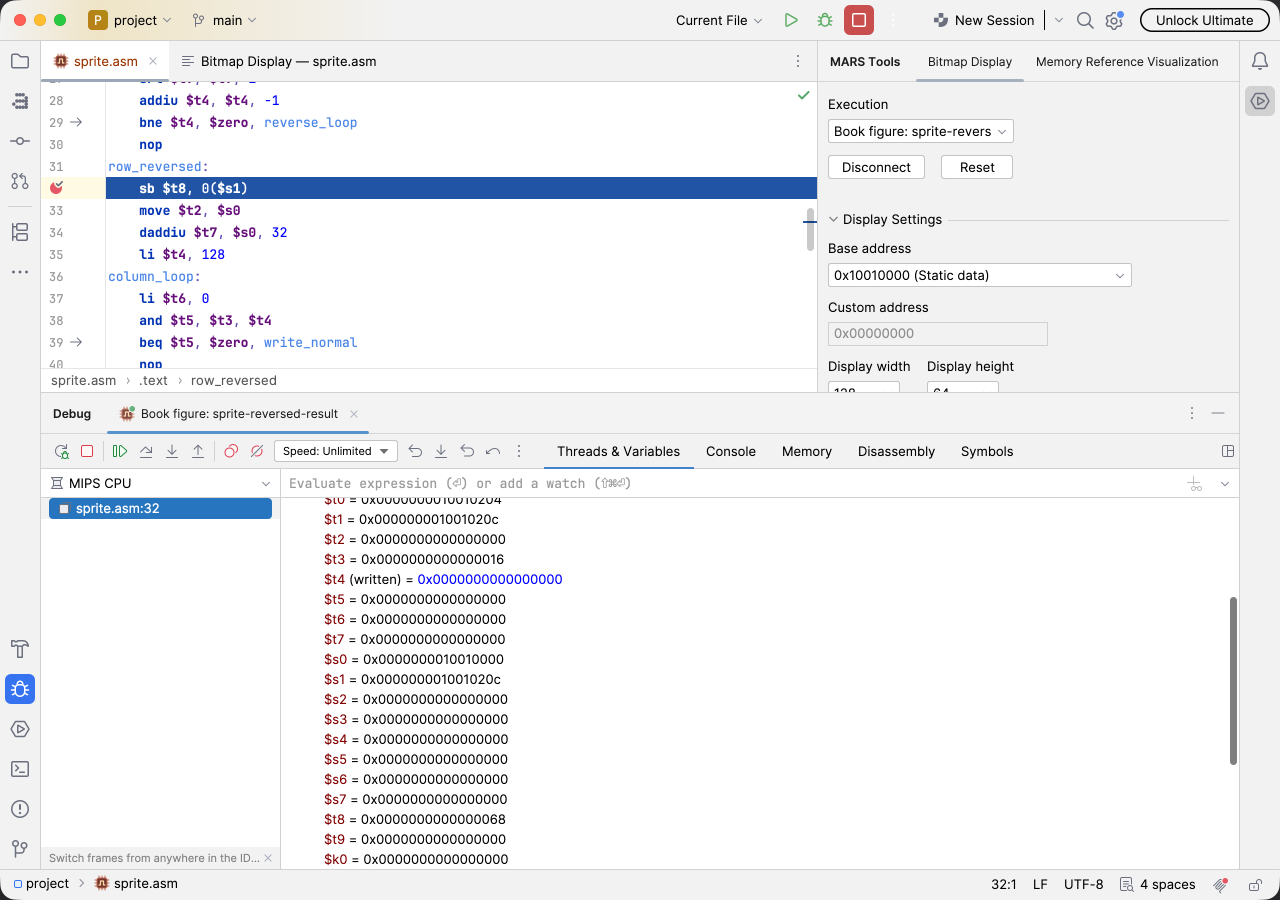
\includegraphics[width=0.53\linewidth,artifact,trim={\MARSreversedreversedLeft{} \MARSreversedreversedBottom{} \MARSreversedreversedRight{} \MARSreversedreversedTop{}},clip]{packages/003-eight-byte-sprite/captures/f02-reversal/result.png}};
    \begin{scope}[shift={(reversed.south west)},x={($(reversed.south east)-(reversed.south west)$)},y={($(reversed.north west)-(reversed.south west)$)}]
      \draw[black,line width=0.7pt] (0.030303030,0.115384615) rectangle (0.969696970,0.884615385);
      \node[draw=black,fill=white,circle,inner sep=1.5pt,font=\footnotesize] at ($(0.030303030,0.884615385)+(-3mm,0)$) {3};
    \end{scope}
    \node[anchor=north west,inner sep=0,font=\small\bfseries] (count-title) at ([yshift=-2mm]reversed.south west) {Eight iterations have consumed the count};
    \node[anchor=north west,inner sep=0] (count) at ([yshift=-1mm]count-title.south west) {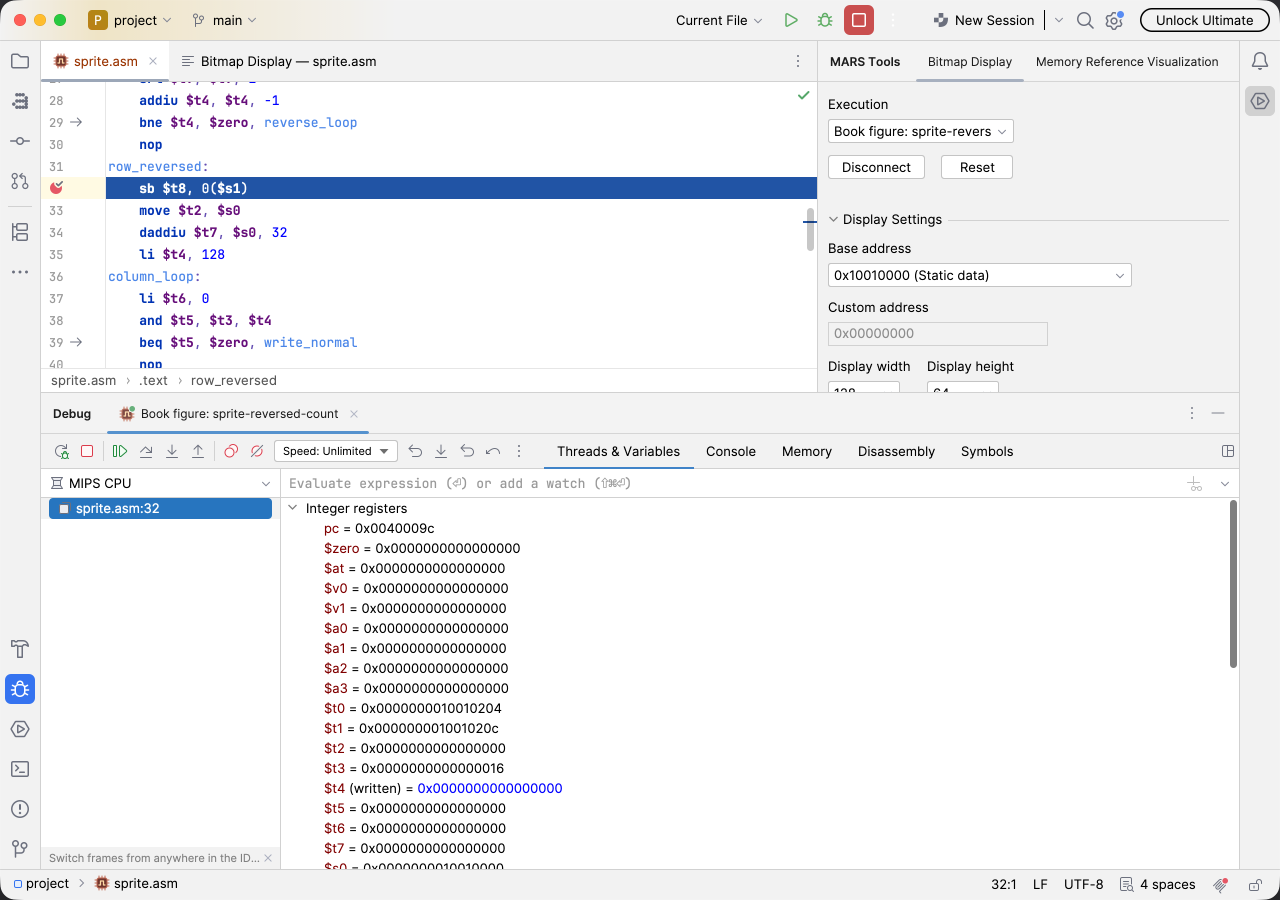
\includegraphics[width=0.53\linewidth,artifact,trim={\MARSreversedcountLeft{} \MARSreversedcountBottom{} \MARSreversedcountRight{} \MARSreversedcountTop{}},clip]{packages/003-eight-byte-sprite/captures/f02-reversal/count.png}};
    \begin{scope}[shift={(count.south west)},x={($(count.south east)-(count.south west)$)},y={($(count.north west)-(count.south west)$)}]
      \draw[black,line width=0.7pt] (0.023529412,0.115384615) rectangle (0.976470588,0.884615385);
      \node[draw=black,fill=white,circle,inner sep=1.5pt,font=\footnotesize] at ($(0.023529412,0.884615385)+(-3mm,0)$) {4};
    \end{scope}
  \end{tikzpicture}
  \par\smallskip
  \begin{minipage}{\linewidth}
    \small
    \begin{enumerate}
      \item The loop has finished, and \texttt{sb \$t8, 0(\$s1)} is the next instruction. At this boundary the reversed value is ready in a register; it has not yet been stored in the output array.
      \item \texttt{\$t3}=\texttt{0x16}, the original row. The reversal consumed the separate working copy in \texttt{\$t9}, preserving this mask for the left half of the display.
      \item \texttt{\$t8}=\texttt{0x68}=104. Read each byte most significant bit first: \texttt{00010110} becomes \texttt{01101000}. Reversing the eight bit positions changes the horizontal order of the cells.
      \item \texttt{\$t4}=0 is the exhausted reversal count. Its initial value was eight. Later code reuses this register as the drawing mask, beginning at 128; the same register has different roles at different boundaries.
    \end{enumerate}
  \end{minipage}
  \caption{The first row after eight reversal iterations, before storing the reversed byte. Three native Debug views share this stop.}
  \label{capture:003-eight-byte-sprite-f02-reversal}
\end{figure}
\par
